\documentclass{article}
\usepackage{tikz}


\tikzstyle{cblue}=[circle, draw, thin,fill=cyan!20, scale=0.8]
\tikzstyle{cempt}=[circle, draw, thin, scale=0.8]


\begin{document}
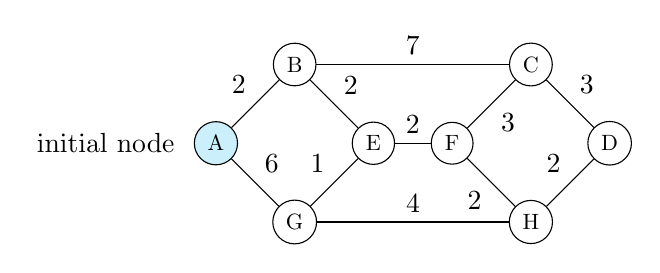
\begin{tikzpicture}[auto, thick, scale=1]

\node[cblue] (n1) at (0,0) {A};
\node at (-1.4,0) {initial node};

\node[cempt] (n2) at (1,1) {B};
\node[cempt] (n3) at (4,1) {C};
\node[cempt] (n4) at (5,0) {D};
\node[cempt] (n5) at (2,0) {E};
\node[cempt] (n6) at (3,0) {F};
\node[cempt] (n7) at (4,-1) {H};
\node[cempt] (n8) at (1,-1) {G};
 
\draw[thin] (n1) -- (n2) node[midway] {2};
\draw[thin] (n2) -- (n3) node[midway] {7};
\draw[thin] (n3) -- (n4) node[midway] {3};
\draw[thin] (n1) -- (n8) node[midway] {6};
\draw[thin] (n8) -- (n7) node[midway] {4};
\draw[thin] (n7) -- (n4) node[midway] {2};
\draw[thin] (n8) -- (n5) node[midway] {1};
\draw[thin] (n2) -- (n5) node[midway] {2};
\draw[thin] (n3) -- (n6) node[midway] {3};
\draw[thin] (n7) -- (n6) node[midway] {2};
\draw[thin] (n5) -- (n6) node[midway] {2};

\end{tikzpicture}
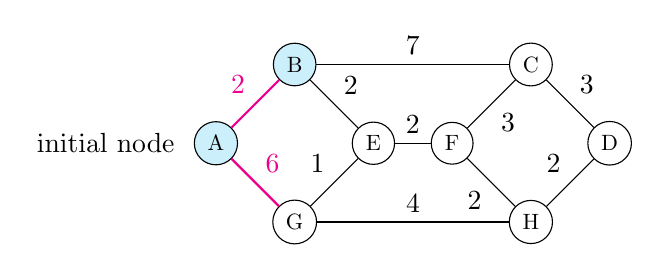
\begin{tikzpicture}[auto, thick, scale=1]

\node[cblue] (n1) at (0,0) {A};
\node at (-1.4,0) {initial node};

\node[cblue] (n2) at (1,1) {B};
\node[cempt] (n3) at (4,1) {C};
\node[cempt] (n4) at (5,0) {D};
\node[cempt] (n5) at (2,0) {E};
\node[cempt] (n6) at (3,0) {F};
\node[cempt] (n7) at (4,-1) {H};
\node[cempt] (n8) at (1,-1) {G};
 
\draw[thick,magenta] (n1) -- (n2) node[midway] {2};
\draw[thin] (n2) -- (n3) node[midway] {7};
\draw[thin] (n3) -- (n4) node[midway] {3};
\draw[thick, magenta] (n1) -- (n8) node[midway] {6};
\draw[thin] (n8) -- (n7) node[midway] {4};
\draw[thin] (n7) -- (n4) node[midway] {2};
\draw[thin] (n8) -- (n5) node[midway] {1};
\draw[thin] (n2) -- (n5) node[midway] {2};
\draw[thin] (n3) -- (n6) node[midway] {3};
\draw[thin] (n7) -- (n6) node[midway] {2};
\draw[thin] (n5) -- (n6) node[midway] {2};

\end{tikzpicture}\\

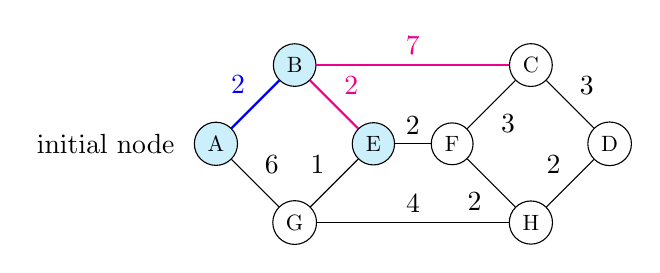
\begin{tikzpicture}[auto, thick, scale=1]

\node[cblue] (n1) at (0,0) {A};
\node at (-1.4,0) {initial node};

\node[cblue] (n2) at (1,1) {B};
\node[cempt] (n3) at (4,1) {C};
\node[cempt] (n4) at (5,0) {D};
\node[cblue] (n5) at (2,0) {E};
\node[cempt] (n6) at (3,0) {F};
\node[cempt] (n7) at (4,-1) {H};
\node[cempt] (n8) at (1,-1) {G};
 
\draw[thick, blue] (n1) -- (n2) node[midway] {2};
\draw[thick, magenta] (n2) -- (n3) node[midway] {7};
\draw[thin] (n3) -- (n4) node[midway] {3};
\draw[thin] (n1) -- (n8) node[midway] {6};
\draw[thin] (n8) -- (n7) node[midway] {4};
\draw[thin] (n7) -- (n4) node[midway] {2};
\draw[thin] (n8) -- (n5) node[midway] {1};
\draw[thick, magenta] (n2) -- (n5) node[midway] {2};
\draw[thin] (n3) -- (n6) node[midway] {3};
\draw[thin] (n7) -- (n6) node[midway] {2};
\draw[thin] (n5) -- (n6) node[midway] {2};

\end{tikzpicture}
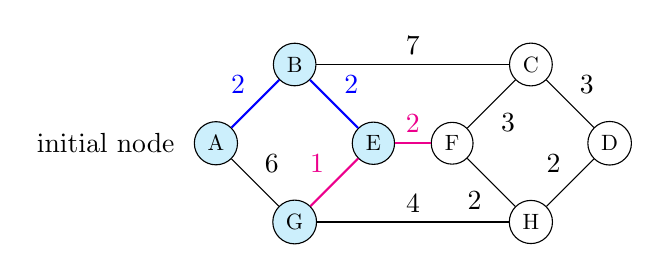
\begin{tikzpicture}[auto, thick, scale=1]

\node[cblue] (n1) at (0,0) {A};
\node at (-1.4,0) {initial node};

\node[cblue] (n2) at (1,1) {B};
\node[cempt] (n3) at (4,1) {C};
\node[cempt] (n4) at (5,0) {D};
\node[cblue] (n5) at (2,0) {E};
\node[cempt] (n6) at (3,0) {F};
\node[cempt] (n7) at (4,-1) {H};
\node[cblue] (n8) at (1,-1) {G};
 
\draw[thick, blue] (n1) -- (n2) node[midway] {2};
\draw[thin] (n2) -- (n3) node[midway] {7};
\draw[thin] (n3) -- (n4) node[midway] {3};
\draw[thin] (n1) -- (n8) node[midway] {6};
\draw[thin] (n8) -- (n7) node[midway] {4};
\draw[thin] (n7) -- (n4) node[midway] {2};
\draw[thick,magenta] (n8) -- (n5) node[midway] {1};
\draw[thick, blue] (n2) -- (n5) node[midway] {2};
\draw[thin] (n3) -- (n6) node[midway] {3};
\draw[thin] (n7) -- (n6) node[midway] {2};
\draw[thick, magenta] (n5) -- (n6) node[midway] {2};

\end{tikzpicture}\\

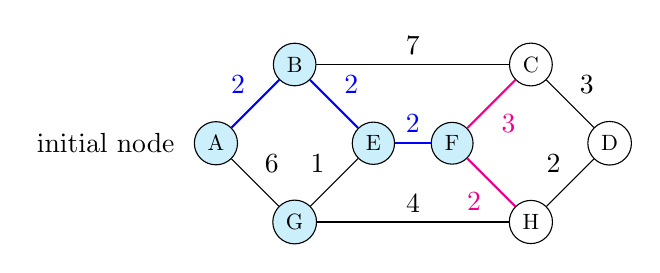
\begin{tikzpicture}[auto, thick, scale=1]

\node[cblue] (n1) at (0,0) {A};
\node at (-1.4,0) {initial node};

\node[cblue] (n2) at (1,1) {B};
\node[cempt] (n3) at (4,1) {C};
\node[cempt] (n4) at (5,0) {D};
\node[cblue] (n5) at (2,0) {E};
\node[cblue] (n6) at (3,0) {F};
\node[cempt] (n7) at (4,-1) {H};
\node[cblue] (n8) at (1,-1) {G};
 
\draw[thick,blue] (n1) -- (n2) node[midway] {2};
\draw[thin] (n2) -- (n3) node[midway] {7};
\draw[thin] (n3) -- (n4) node[midway] {3};
\draw[thin] (n1) -- (n8) node[midway] {6};
\draw[thin] (n8) -- (n7) node[midway] {4};
\draw[thin] (n7) -- (n4) node[midway] {2};
\draw[thin] (n8) -- (n5) node[midway] {1};
\draw[thick, blue] (n2) -- (n5) node[midway] {2};
\draw[thick,magenta] (n3) -- (n6) node[midway] {3};
\draw[thick,magenta] (n7) -- (n6) node[midway] {2};
\draw[thick,blue] (n5) -- (n6) node[midway] {2};

\end{tikzpicture}
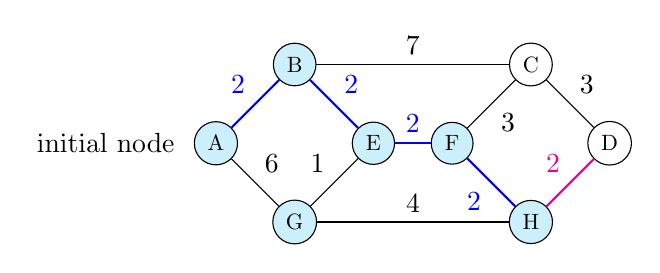
\begin{tikzpicture}[auto, thick, scale=1]

\node[cblue] (n1) at (0,0) {A};
\node at (-1.4,0) {initial node};

\node[cblue] (n2) at (1,1) {B};
\node[cempt] (n3) at (4,1) {C};
\node[cempt] (n4) at (5,0) {D};
\node[cblue] (n5) at (2,0) {E};
\node[cblue] (n6) at (3,0) {F};
\node[cblue] (n7) at (4,-1) {H};
\node[cblue] (n8) at (1,-1) {G};
 
\draw[thick,blue] (n1) -- (n2) node[midway] {2};
\draw[thin] (n2) -- (n3) node[midway] {7};
\draw[thin] (n3) -- (n4) node[midway] {3};
\draw[thin] (n1) -- (n8) node[midway] {6};
\draw[thin] (n8) -- (n7) node[midway] {4};
\draw[thick,magenta] (n7) -- (n4) node[midway] {2};
\draw[thin] (n8) -- (n5) node[midway] {1};
\draw[thick, blue] (n2) -- (n5) node[midway] {2};
\draw[thin] (n3) -- (n6) node[midway] {3};
\draw[thick,blue] (n7) -- (n6) node[midway] {2};
\draw[thick,blue] (n5) -- (n6) node[midway] {2};

\end{tikzpicture}

\end{document}
